\chapter{Avaliações do Protótipo de Papel}

\section{Relatório Consolidado - Avaliação 1 Protótipo de Papel}

\textbf{Data da avaliação:} 05/04/2015

\textbf{Objetivo:}
O objetivo dessa avaliação consistiu na elicitação de requisitos através de um teste feito em um protótipo de papel.

\textbf{Método:}
O método empregado foi o Quick and Dirty \cite{preece}. Foi realizada em um ambiente informal e foi realizada no início do projeto.

\textbf{Usuários e perfil:}
Essa primeira avaliação foi realizada apenas com 1 usuário que se encaixava no público alvo da aplicação proposta. Foi escolhido apenas 1 usuário, pois o objetivo era obter uma rápida avaliação para elicitação de requisitos.

\textbf{Dados coletados:}
Ideias do usuário para uma tela.
% Colocar imagem

\textbf{Lista dos problemas encontrados:}
\begin{figure}[h!]
  \centering
    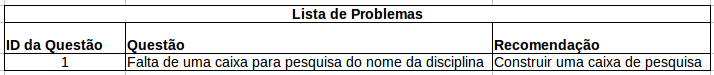
\includegraphics[keepaspectratio=true, scale=0.7]{figuras/problema1.png}
  \caption{Lista de problemas da avaliação}
\end{figure}

\textbf{Planejamento para a próxima versão do protótipo:}
Levando em consideração os problemas encontrados será construída uma nova versão do protótipo. 
\vfill
\pagebreak

\section{Relatório Consolidado - Avaliação 2 Protótipo de Papel}

\textbf{Data da avaliação:} 08/05/2015

\textbf{Objetivo:}
O objetivo dessa avaliação consistiu na elicitação de requisitos através de um teste feito em um protótipo de papel.

\textbf{Método:}
O método empregado foi o \textit{Quick and Dirty} \cite{preece}. Foi realizada em um ambiente informal e foi realizada na segunda versão do protótipo construído.

\textbf{Usuários e perfil:}
Essa avaliação foi realizada com 3 usuários que se encaixavam no público alvo da aplicação proposta. Com a continuação do uso do método \textit{Quick and Dirty} os avaliadores optaram por não avaliar com muitos usuários, pois o objetivo ainda era elicitar requisitos. Assim, para não concentrar essa última avaliação do protótipo de papel em apenas um usuário, foi optado pela escolha de 3 usuários.

\textbf{Dados coletados:}
Ideias do usuário para uma tela.
% Colocar imagem

\textbf{Lista dos problemas encontrados:}
\begin{figure}[h!]
  \centering
    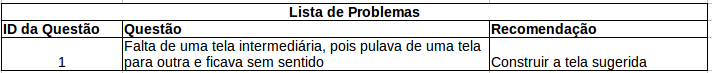
\includegraphics[keepaspectratio=true, scale=0.7]{figuras/problema2.png}
  \caption{Lista de problemas da avaliação}
\end{figure}

\textbf{Planejamento para a próxima versão do protótipo:}
Levando em consideração os requisitos levantados será construída uma nova versão do protótipo de papel.

\vfill
\pagebreak
\section{Relatório Consolidado - Avaliação 3 Protótipo de Papel}

\textbf{Data da avaliação:} 03/06/2015

\textbf{Objetivo:}
O objetivo dessa avaliação consistiu no teste da estabilidade do protótipo de papel.

\textbf{Método:}
O método empregado foi a observação direta \cite{preece}. Foi realizada em um ambiente informal e foi realizada na terceira versão do protótipo construído.

\textbf{Usuários e perfil:}
Essa avaliação foi realizada com 5 usuários que se encaixavam no público alvo da aplicação proposta. 

\textbf{Dados coletados:}
...

\textbf{Lista dos problemas encontrados:}
\begin{figure}[h!]
  \centering
    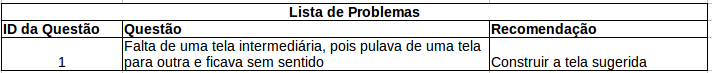
\includegraphics[keepaspectratio=true, scale=0.7]{figuras/problema2.png}
  \caption{Lista de problemas da avaliação}
\end{figure}

\textbf{Planejamento para a próxima versão do protótipo:}
O protótipo será repassado para uma ferramenta.
 